



\begin{document}

\begin{multicols}{2}

из них: \(m=0, 1, 3, 5; -2, -4\). Вычисляя при этих значенях лувую и правую части уранения $(2)$, получаем таблицу 
\begin{tabular}{
|>{\centering}p{1cm}|
p{0.3cm}<{\centering}|
p{0.3cm}<{\centering}|
p{0.3cm}<{\centering}|
p{0.3cm}<{\centering}|
p{0.3cm}<{\centering}|
p{0.3cm}<{\centering}|
} %l - по лувому краю с - по правому к - по левому
\hline
$m$ & $0$ & $1$ & $3$ & $5$\vspace{5pt} & $-2$ & $-4$ \\
$sin$$\frac{f}{r}$
&0 &$\frac{1}{2}$ &1 &$\frac{1}{2}$  &$\frac{\sqrt{3}}{2}$  &$\frac{\sqrt{3}}{2}$ \vspace{0.5pt} \\
\(sin\frac{f}{r}\) & 1& 1& 1& 1& 1& 1 \vspace{5pt}\\
\hline

\end{tabular}

из которой получаем искомые решения: $m=0,1,5$ т.е.


\begin{centering}
\vspace{10pt}

$x=0$,  $\frac{\pi}{6}$, $\frac{5\pi}{6}$.    $(3)$


\end{centering}
\vspace{10pt}
Три значения $(3)$ и дают полное решение задачи, так как решение серии $(a)$ давало значение $x=0$, уже включенное
в $(3)$

Отметим, что таким же образом, путем перебора, можно проверить и серию $(a)$.

При решении этой задачи характерной ошибкой была следующее: многие забывали, что решение должно удовлетворять всем условиям задачи \textit{одновременно}, a зачастую просто не понимали этого. Некоторые
ораничивались тем, что решали одно из уравнений и совершали отбор решений по неравенству, другие комбинировали 
уравнения и решили в конце концов, не эквивалентное предложеной системе.

\begin{center}
Задача 4
\end{center}

Пусть $ABCD-$ данный четыречугольник, $AB=\frac{\sqrt[7]{a^2-\sqrt{ab+\sqrt[\frac{3}{4}]{b^2}}}}{a^2-a^2+ab+a^2-2ab+b^{sina}}$. Прямогольные проекции любого многоугольника на параллельне плоскости равны между собой; поэтому проведем плоскости $P_1$ и $P_2$ параллельные исходным плоскостям, ч е р е з \hspace{2pt} в е р ш и н у $A$ и в дальнейшем будем говорить о проекциях четырехуголника именно на эти плоскости.

Для каждой точки $M$ пространства мы будем обозначать через $M_1,M_2$ и $M_3$ проекции точки $M$ соответсвенно на плоскость $P_1$, плоскость $P_2$ и прямоую пересечения $P_1$ и $P_2$; очевидно, 
$MM_1=M_2M_3$ и $MM_2=M_1M_3$. По принятому построению плоскостей $P_1$ и $P_2$ все три проекции точки $A(A_1, A_2$ и $A_3)$ совподают с $A$; по условию задаи $AB_1C_1D_1$ и $A_2B_2C_2D-$
квадраты со стороной 2.

\center{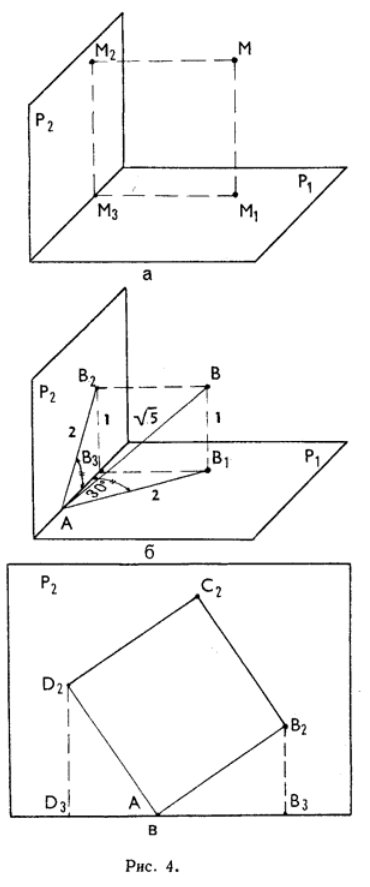
\includegraphics[width=6cm]{Picture}{\centering}}
\end{multicols}
\end{document}